\documentclass[a4paper]{slides}

\usepackage{tikz}
\usepackage{geometry}

\usepackage[scaled]{helvet}
\usepackage[T1]{fontenc}

% Set Layout
\geometry{
    a4paper,
    left=25mm,
    right=25mm,
    top=25mm,
    bottom=25mm
}

\begin{document}

\fontsize{15}{1.5}\textbf{Bitte in Schreibrichtung die Großbuchstaben von A bis Z eintragen}

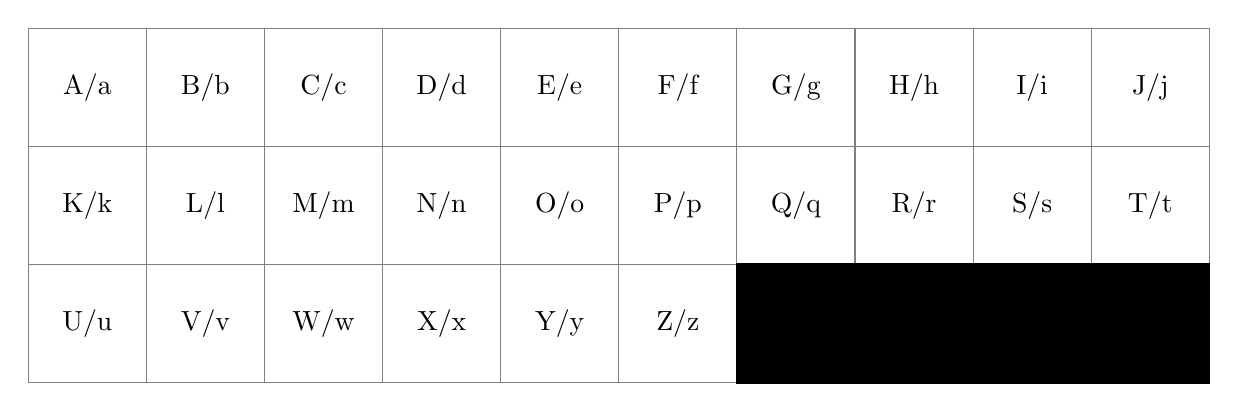
\begin{tikzpicture}[thick, scale=1.5]
    \draw[step=1cm,gray,thin] (0,0) grid (10,3);
    % letter
    \node[anchor = center] () at (0.5,2.5){A/a};
    \node[anchor = center] () at (1.5,2.5){B/b};
    \node[anchor = center] () at (2.5,2.5){C/c};
    \node[anchor = center] () at (3.5,2.5){D/d};
    \node[anchor = center] () at (4.5,2.5){E/e};
    \node[anchor = center] () at (5.5,2.5){F/f};
    \node[anchor = center] () at (6.5,2.5){G/g};
    \node[anchor = center] () at (7.5,2.5){H/h};
    \node[anchor = center] () at (8.5,2.5){I/i};
    \node[anchor = center] () at (9.5,2.5){J/j};
    \node[anchor = center] () at (0.5,1.5){K/k};
    \node[anchor = center] () at (1.5,1.5){L/l};
    \node[anchor = center] () at (2.5,1.5){M/m};
    \node[anchor = center] () at (3.5,1.5){N/n};
    \node[anchor = center] () at (4.5,1.5){O/o};
    \node[anchor = center] () at (5.5,1.5){P/p};
    \node[anchor = center] () at (6.5,1.5){Q/q};
    \node[anchor = center] () at (7.5,1.5){R/r};
    \node[anchor = center] () at (8.5,1.5){S/s};
    \node[anchor = center] () at (9.5,1.5){T/t};
    \node[anchor = center] () at (0.5,0.5){U/u};
    \node[anchor = center] () at (1.5,0.5){V/v};
    \node[anchor = center] () at (2.5,0.5){W/w};
    \node[anchor = center] () at (3.5,0.5){X/x};
    \node[anchor = center] () at (4.5,0.5){Y/y};
    \node[anchor = center] () at (5.5,0.5){Z/z};

    % black square
    \filldraw[fill=black, draw=black] (6,0) rectangle (7,1);
    \filldraw[fill=black, draw=black] (7,0) rectangle (8,1);
    \filldraw[fill=black, draw=black] (8,0) rectangle (9,1);
    \filldraw[fill=black, draw=black] (9,0) rectangle (10,1);
\end{tikzpicture}

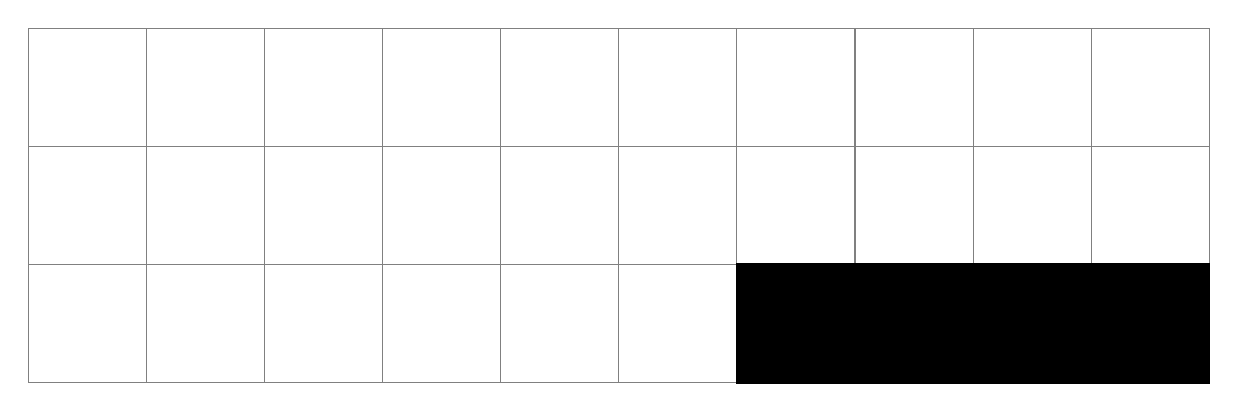
\begin{tikzpicture}[thick, scale=1.5]
    \draw[step=1cm,gray,thin] (0,0) grid (10,3);
    \filldraw[fill=black, draw=black] (6,0) rectangle (7,1);
    \filldraw[fill=black, draw=black] (7,0) rectangle (8,1);
    \filldraw[fill=black, draw=black] (8,0) rectangle (9,1);
    \filldraw[fill=black, draw=black] (9,0) rectangle (10,1);
\end{tikzpicture}

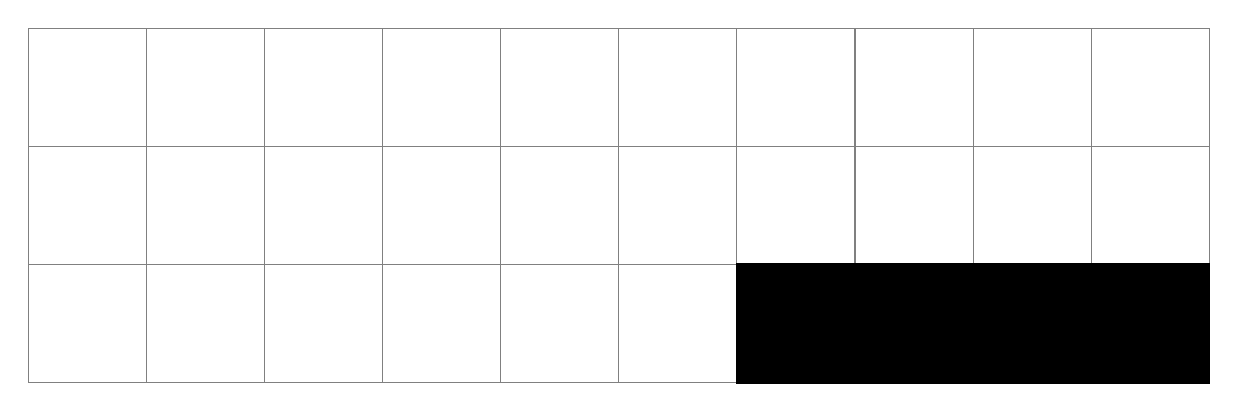
\begin{tikzpicture}[thick, scale=1.5]
    \draw[step=1cm,gray,thin] (0,0) grid (10,3);
    \filldraw[fill=black, draw=black] (6,0) rectangle (7,1);
    \filldraw[fill=black, draw=black] (7,0) rectangle (8,1);
    \filldraw[fill=black, draw=black] (8,0) rectangle (9,1);
    \filldraw[fill=black, draw=black] (9,0) rectangle (10,1);
\end{tikzpicture}

\fontsize{14}{1.5}\textbf{Bitte in jede Reihe die Zahlen von 0 bis 9 eintragen }

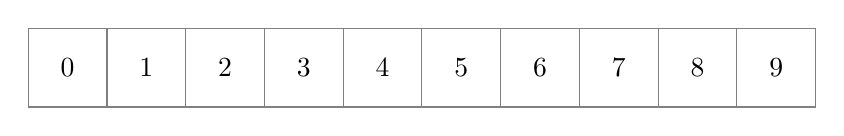
\begin{tikzpicture}[thick, scale=1]
    \draw[step=1cm,gray,thin] (0,0) grid (10,1);
    \node[anchor = center] () at (0.5,0.5){0};
    \node[anchor = center] () at (1.5,0.5){1};
    \node[anchor = center] () at (2.5,0.5){2};
    \node[anchor = center] () at (3.5,0.5){3};
    \node[anchor = center] () at (4.5,0.5){4};
    \node[anchor = center] () at (5.5,0.5){5};
    \node[anchor = center] () at (6.5,0.5){6};
    \node[anchor = center] () at (7.5,0.5){7};
    \node[anchor = center] () at (8.5,0.5){8};
    \node[anchor = center] () at (9.5,0.5){9};
\end{tikzpicture}

\begin{tikzpicture}[thick, scale=1.5]
    \draw[step=1cm,gray,thin] (0,0) grid (10,3);
\end{tikzpicture}

\end{document}
